\documentclass[14pt,beamer]{beamer}
\usepackage[brazilian]{babel}
\usepackage[utf8]{inputenc} % Codificação UTF-8
\usepackage[T2A,T1]{fontenc} % Pacote de hifenização
\usepackage{graphicx} % Imagens
\usepackage{tabularx}
\usepackage{booktabs} 
\usepackage{color}
\usepackage{textcomp}
\usepackage{multicol}
\usefonttheme{professionalfonts}

%###############################################
%         PRECISA TER O RA NOS SLIDES?
%###############################################

\newcommand\cyrtext[1]{{\fontencoding{T2A}\selectfont #1}}

\usepackage{tabularx,colortbl} % Cores nas tabelas


\setbeamertemplate{title page}[default][colsep=-5bp,rounded=true]

\usetheme[height=15pt]{Berkeley}
\usecolortheme[RGB={26,89,142}]{structure} 
\setbeamertemplate{navigation symbols}{}
\setbeamertemplate{blocks}[rounded][shadow=true] 

\defbeamertemplate*{footline}{infolines theme without institution}
{
  \leavevmode%
  \hbox{%
  \begin{beamercolorbox}[wd=.5\paperwidth,ht=2.25ex,dp=1ex,center]{title in head/foot}%
    \usebeamerfont{title in head/foot}\insertshorttitle
  \end{beamercolorbox}%
  \begin{beamercolorbox}[wd=.5\paperwidth,ht=2.25ex,dp=1ex,right]{date in head/foot}%
    \usebeamerfont{date in head/foot}\insertshortdate{}\hspace*{7em}
    \insertframenumber{} / \inserttotalframenumber\hspace*{2ex}
  \end{beamercolorbox}}%
  \vskip0pt%
}



\title[Doutor Pecúlio]{Doutor Pecúlio - App para compras pelo menor preço}

\author[Carlos, Lucas e Paulo Roberto]{ \normalsize Carlos A. O. de Souza Junior \footnotesize{(570101439)} \\ 
		\and \normalsize Lucas J. C. Lorenzetti \footnotesize{(570091430)} \\ 
		\and \normalsize Paulo R. Urio \footnotesize{(570091403)} }
%\institute[]{
%  Departamento de Ciência da Computação \\
%  Universidade Estadual do Centro-Oeste \\
%  Guarapuava, Brasil
%}
\institute[]{
    \vspace{10px}~ \\
    
\includegraphics[scale=0.2]{imagens/logo} \\
  {\rmfamily\scshape Universidade Estadual do Centro-Oeste}
}
\date{}

     


\makeatletter
\setlength{\beamer@headheight}{1cm}

\setbeamertemplate{footline}
{
  \leavevmode%
  \hbox{%
  \begin{beamercolorbox}[wd=.333333\paperwidth,ht=2.25ex,dp=1ex,center]{author in head/foot}%
    \usebeamerfont{author in head/foot}\insertshortauthor~~\beamer@ifempty{\insertshortinstitute}{}{\insertshortinstitute}
  \end{beamercolorbox}%
  \begin{beamercolorbox}[wd=.333333\paperwidth,ht=2.25ex,dp=1ex,center]{title in head/foot}%
    \usebeamerfont{title in head/foot}\insertshorttitle
  \end{beamercolorbox}%
  \begin{beamercolorbox}[wd=.333333\paperwidth,ht=2.25ex,dp=1ex,right]{date in head/foot}%
    \usebeamerfont{date in head/foot}\insertshortdate{\today}\hspace*{2em}
    \insertframenumber{} / \inserttotalframenumber\hspace*{2ex} 
  \end{beamercolorbox}}%
  \vskip0pt%
}

\makeatother

\begin{document}
	\begin{frame}
		\titlepage
	\end{frame}

\begin{frame}
	\frametitle{Conteúdo}
    \begin{multicols}{2}
        \small
        \tableofcontents[currentsection,hideothersubsections]
    \end{multicols}
\end{frame}

% %%%%%%%%%%%%%%%%%%%%%%%%%%%%%%%% section %%%%%%%%%%%%%%%%%%%%%%%%%%%%%%%%%%%%
% -------------------------------- section ------------------------------------
\section{Introdução}


% --------------------------------- slide -------------------------------------
\begin{frame}
	\frametitle{Conteúdo}
    \begin{multicols}{2}
        \small
        \tableofcontents[currentsection,hideothersubsections]
    \end{multicols}
\end{frame}

% --------------------------------- slide -------------------------------------
\begin{frame}
	\frametitle{Assistente Pessoal Inteligente}
    \framesubtitle{Definições}

    \begin{block}{\emph{Intelligent Personal Assistant} (IPA)}
        Agente de \emph{software} que pode realizar tarefas e
        serviços para um indivíduo de forma personalizada,
        acessando APIs.
    \end{block}
    
    \begin{block}{\emph{Application Programming Interface} (API)}
        Integração com interfaces públicas foi popularizada com a proliferação
        de aplicativos móveis com acesso à \emph{internet}.
    \end{block}
    
    Exemplos de IPAs:
    \begin{itemize}
        \item Google Now; e
        \item Apple Siri.
    \end{itemize}
\end{frame}

% --------------------------------- slide -------------------------------------
\begin{frame}
	\frametitle{Assistente Pessoal Inteligente}
    \framesubtitle{Exemplo}

    \begin{block}{Google Now}
        Agrupa personalizadamente os dados em tempo real do:
        \begin{itemize}
            \item Clima;
            \item tráfego;
            \item notícias;
            \item ações;
            \item preços de varejo;
            \item etc.
        \end{itemize}
    \end{block}
\end{frame}

% --------------------------------- slide -------------------------------------
\begin{frame}
	\frametitle{Assistente Pessoal Inteligente}
    \framesubtitle{Exemplo}

    \begin{block}{Apple Siri}
        \begin{itemize}
            \item Assistente cognitivo inteligente;
            \item utiliza linguagem natural;
            \item redireciona tarefas à outros IPAs; e
            \item utiliza IA para conversar com o usuário.
        \end{itemize}
    \end{block}
\end{frame}


% --------------------------------- slide -------------------------------------
\begin{frame}
	\frametitle{Assistente Pessoal Inteligente}
    \framesubtitle{Objetivo}

    \begin{block}{Objetivo}
        Nosso trabalho é voltado ao desenvolvimento 
        \begin{itemize}
            \item da prévia de um agente inteligente;
            \item para consultas de preços.
        \end{itemize}
        Para o protótipo desenvolvido, foram feitos
        \begin{itemize}
            \item Casos de uso;
            \item Cenários;
            \item Personas;
            \item Análise de requisitos; e
            \item Avaliação da interface do protótipo.
        \end{itemize}
    \end{block}
\end{frame}

% %%%%%%%%%%%%%%%%%%%%%%%%%%%%%%%% section %%%%%%%%%%%%%%%%%%%%%%%%%%%%%%%%%%%%
% -------------------------------- section ------------------------------------
\section{Doutor Pecúlio}

% --------------------------------- slide -------------------------------------
\begin{frame}
	\frametitle{Conteúdo}
    \begin{multicols}{2}
        \small
        \tableofcontents[currentsection,hideothersubsections]
    \end{multicols}
\end{frame}

% --------------------------------- slide -------------------------------------
\begin{frame}
	\frametitle{O aplicativo}
    
	\vspace{-30px}
	\begin{columns}
		\begin{column}{.3\textwidth}
			\begin{figure}
				
\includegraphics[scale=.15]{imagens/docpig}
			\end{figure}
		\end{column}%
		\hfill%
		\begin{column}{9\textwidth}
			\large{\textbf{Doutor Pecúlio}}
		\end{column}%
	\end{columns}
	
	\vspace{10px}
	\begin{itemize}
        \item Assistente inteligente;
        \item Para Android;
		\item Consulta preços em catálogos de
			\begin{itemize}
				\item lojas próximas; e
				\item lojas virtuais. 	
			\end{itemize}
		\item Busca feita através de uma foto
			\begin{itemize}
				\item da capa;
				\item do código de barras; e
                \item do código QR (\emph{Quick Response})
			\end{itemize}
	\end{itemize}
\end{frame}


% --------------------------------- slide -------------------------------------
\begin{frame}
	\frametitle{O aplicativo}
    \framesubtitle{Foco da aplicação}
	
	\vspace{-30px}
	\begin{columns}
		\begin{column}{.3\textwidth}
			\begin{figure}
				
\includegraphics[scale=.15]{imagens/docpig}
			\end{figure}
		\end{column}%
		\hfill%
		\begin{column}{9\textwidth}
			\large{\textbf{Doutor Pecúlio}}
		\end{column}%
	\end{columns}
	
	\vspace{10px}
    O aplicativo é voltado para identificar imagens de
	\begin{itemize}
        \item Livros;
        \item CDs, DVDs, Blu-ray;
        \item mídias para PCs; e
        \item mídas para consoles de \emph{videogame}.
	\end{itemize}
\end{frame}



% --------------------------------- slide -------------------------------------
\begin{frame}
	\frametitle{O aplicativo}
    \framesubtitle{Motivação}
	
	\vspace{-30px}
	\begin{columns}
		\begin{column}{.3\textwidth}
			\begin{figure}
				
\includegraphics[scale=.15]{imagens/docpig}
			\end{figure}
		\end{column}%
		\hfill%
		\begin{column}{9\textwidth}
			\large{\textbf{Doutor Pecúlio}}
		\end{column}%
	\end{columns}

	\vspace{10px}
    \begin{columns}
        \begin{column}{.8\textwidth}
            \begin{itemize}
                \item Os aplicativos atuais necessitam da entrada manual
                    \begin{itemize}
                    \item do identificador ISBN;
                    \item do nome do autor;
                    \item do título; ou 
                    \item de detalhes edição e editora.
                    \end{itemize}
            \end{itemize}
        \end{column}
        \begin{column}{.2\textwidth}
            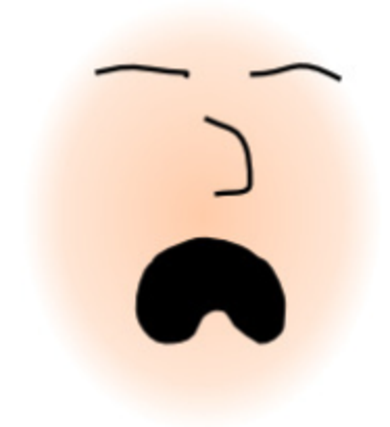
\includegraphics[scale=.3]{imagens/LixoSono}
        \end{column}
    \end{columns}
\end{frame}



% --------------------------------- slide -------------------------------------
\begin{frame}
	\frametitle{O aplicativo}
    \framesubtitle{Motivação}
	
	\vspace{-30px}
	\begin{columns}
		\begin{column}{.3\textwidth}
			\begin{figure}
				
\includegraphics[scale=.15]{imagens/docpig}
			\end{figure}
		\end{column}%
		\hfill%
		\begin{column}{9\textwidth}
			\large{\textbf{Doutor Pecúlio}}
		\end{column}%
	\end{columns}
	
	\vspace{20px}
	Através de técnicas visão computacional
            \begin{itemize}
            \item \emph{Content-Based Image Retrieval} (CBIR); e
            \item \emph{Implicit Concept-Based Image Indexing and Retrieval} (ICIIR);
            \end{itemize}
    é possível utilizar fotos para realizar buscas.
\end{frame}


% --------------------------------- slide -------------------------------------
\begin{frame}
	\frametitle{O aplicativo}
    \framesubtitle{Público alvo}
	
	\vspace{-30px}
	\begin{columns}
		\begin{column}{.3\textwidth}
			\begin{figure}
				
\includegraphics[scale=.15]{imagens/docpig}
			\end{figure}
		\end{column}%
		\hfill%
		\begin{column}{9\textwidth}
			\large{\textbf{Doutor Pecúlio}}
		\end{column}%
	\end{columns}
	
    \begin{block}{Público alvo}
        \begin{itemize}
            \item Utiliza um \emph{smartphone} moderno;
            \item com câmera interna; e
            \item conexão à \emph{internet}.
        \end{itemize}
        Imagina-se que o usuário utilizará em situações corriqueiras, 
        onde o aplicativo
        \begin{itemize}
            \item Não precise de atenção exclusiva; e
            \item Tenha pouco impacto na atividade atual;
        \end{itemize}
    \end{block}
\end{frame}



% %%%%%%%%%%%%%%%%%%%%%%%%%%%%%%%% section %%%%%%%%%%%%%%%%%%%%%%%%%%%%%%%%%%%%
% -------------------------------- section ------------------------------------
\section{Metas}

% --------------------------------- slide -------------------------------------
\begin{frame}
	\frametitle{Conteúdo}
    \begin{multicols}{2}
        \small
        \tableofcontents[currentsection,hideothersubsections]
    \end{multicols}
\end{frame}

\subsection{Usabilidade}
% --------------------------------- slide -------------------------------------
\begin{frame}
	\frametitle{Metas de usabilidade}

No contexto de desenvolvimento móvel, planejamos manter o foco em
\begin{description}
\item[Aprendizado] Curva de aprendizagem tênue;
\item[Eficiência] Rápido de usar; e
\item[Ergonomia] Fácil de navegar.
\end{description}

\end{frame}

\subsection{Experiência}
% --------------------------------- slide -------------------------------------
\begin{frame}
	\frametitle{Metas de experiência do usuário}

Como metas de experiência, desejamos que seja
\begin{description}
\item[Prestativo] Útil ao usuário;
\item[Motivador] Causar interesse em utilizar;
\item[Recompensador] Garantir que o usuário volte a interagir novamente; e
\item[Agradabilidade] Taxa baixa de erros de consulta.
\end{description}

\end{frame}

% %%%%%%%%%%%%%%%%%%%%%%%%%%%%%%%% section %%%%%%%%%%%%%%%%%%%%%%%%%%%%%%%%%%%%
% -------------------------------- section ------------------------------------
\section{Cenários}

% --------------------------------- slide -------------------------------------
\begin{frame}
	\frametitle{Conteúdo}
    \begin{multicols}{2}
        \small
        \tableofcontents[currentsection,hideothersubsections]
    \end{multicols}
\end{frame}

\subsection{Cenário 1}
% --------------------------------- slide -------------------------------------
\begin{frame}
	\frametitle{Cenários}
	\framesubtitle{Cenário 1}

    \begin{block}{Cenário}
    Uma tentativa bem sucedida de busca de um produto a partir da foto da câmera
    interna do \emph{smartphone}, a qual é utilizada para tirar uma foto da capa de um livro de
    interesse do usuário. O dispositivo já está conectado à uma rede WiFi.
    \end{block}
\end{frame}

\subsection{Cenário 2}
% --------------------------------- slide -------------------------------------
\begin{frame}
	\frametitle{Cenários}
	\framesubtitle{Cenário 2}

    \begin{block}{Cenário}
    Uma tentativa mal sucedida de busca de um produto a partir da
    foto da câmera interna do \emph{smartphone}, a qual é utilizada para
    tirar uma foto do código de barras de um DVD de interesse do usuário.  O dispositivo
    já está conectado à uma rede WiFi.
    \end{block}
\end{frame}

\subsection{Cenário 3}
% --------------------------------- slide -------------------------------------
\begin{frame}
	\frametitle{Cenários}
	\framesubtitle{Cenário 3}

    \begin{block}{Cenário}
    Acesso à uma busca já realizada anteriormente.  O dispositivo
    não precisa estar conectado à WiFi.
    \end{block}
\end{frame}

% %%%%%%%%%%%%%%%%%%%%%%%%%%%%%%%% section %%%%%%%%%%%%%%%%%%%%%%%%%%%%%%%%%%%%
% -------------------------------- section ------------------------------------
\section{Personas}

% --------------------------------- slide -------------------------------------
\begin{frame}
	\frametitle{Conteúdo}
    \begin{multicols}{2}
        \small
        \tableofcontents[currentsection,hideothersubsections]
    \end{multicols}
\end{frame}
\subsection{Persona 1}

% --------------------------------- slide -------------------------------------
\begin{frame}
	\frametitle{Personas}
    \framesubtitle{Persona 1}

    \textbf{Nome:} Eduardo H. de Mello \\
    \textbf{Idade:} 24 anos \\

    \begin{itemize}
        \item Formado em Arquitetura e Urbanismo;
        \item Mudou para Curitiba -- PR para mestrado;
        \item Planeja realizar compras na cidade de Curitiba -- PR:
        \begin{itemize}
            \item A procura do melhor preço em todas as lojas factíveis
                é inexequível.
        \end{itemize}
    \end{itemize}
\end{frame}

\subsection{Persona 2}
% --------------------------------- slide -------------------------------------
\begin{frame}
	\frametitle{Personas}
    \framesubtitle{Persona 2}

    \textbf{Nome:} Clotilde Van Halen \\
    \textbf{Idade:} 43 anos \\

    \begin{itemize}
        \item mulher bem sucedida, chefe de família, 
            presidente do grupo de leitura do bairro e gerente geral de uma 
            agência bancária;
        \item Possui conhecimento de operação de sistemas computacionais;
        \item Formada em Ciências Econômicas;
        \item Tem interesse em tecnologias recentes.
    \end{itemize}
\end{frame}
\subsection{Persona 3}

% --------------------------------- slide -------------------------------------
\begin{frame}
	\frametitle{Personas}
    \framesubtitle{Persona 3}

    \textbf{Nome:} Sirlei da Silva \\
    \textbf{Idade:} 57 anos \\

    \begin{itemize}
        \item Aposentado;
        \item Tem hábito de ir à locadora ver as novidades do cinema;
        \item Mora em uma megalópole;
        \item Utiliza um GPS para não se perder, porém não o domina.
    \end{itemize}
\end{frame}

% %%%%%%%%%%%%%%%%%%%%%%%%%%%%%%%% section %%%%%%%%%%%%%%%%%%%%%%%%%%%%%%%%%%%%
% -------------------------------- section ------------------------------------
\section{Casos de uso}

% --------------------------------- slide -------------------------------------
\begin{frame}
	\frametitle{Conteúdo}
    \begin{multicols}{2}
        \small
        \tableofcontents[currentsection,hideothersubsections]
    \end{multicols}
\end{frame}

% --------------------------------- slide -------------------------------------
\begin{frame}
	\frametitle{Casos de uso}
    
    \begin{figure}
        \centering
        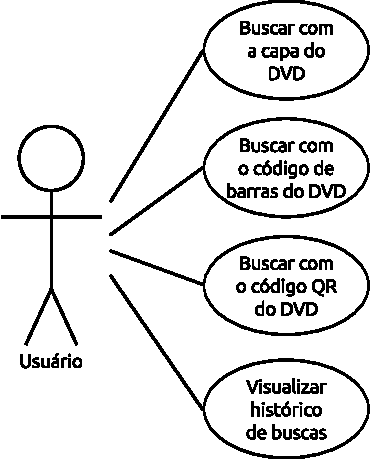
\includegraphics[scale=1]{imagens/caso1.pdf}
    \end{figure}
\end{frame}

% %%%%%%%%%%%%%%%%%%%%%%%%%%%%%%%% section %%%%%%%%%%%%%%%%%%%%%%%%%%%%%%%%%%%%
% -------------------------------- section ------------------------------------
\section{Requisitos}

% --------------------------------- slide -------------------------------------
\begin{frame}
	\frametitle{Conteúdo}
    \begin{multicols}{2}
        \small
        \tableofcontents[currentsection,hideothersubsections]
    \end{multicols}
\end{frame}

% --------------------------------- slide -------------------------------------
\begin{frame}
	\frametitle{Requisitos do sistema}

    \begin{block}{Funcionais}
        \begin{itemize}
            \item Integração com as câmeras internas do \emph{smartphone};
            \item integração com as APIs de compartilhamento de multimídia;
            \item integração com a API GeoIP; e
            \item integração com os serviços de lojas virtuais (Amazon.com, Livraria
                Saraiva, Livrarias Curitiba, Livraria Chain, Submarino.com.br).
        \end{itemize}
    \end{block}
\end{frame}

% --------------------------------- slide -------------------------------------
\begin{frame}
	\frametitle{Requisitos do sistema}

    \begin{block}{Não funcionais}
        \begin{itemize}
            \item Acesso à \emph{internet};
            \item visualização do histórico de buscas; e
            \item acesso ao catálogo de lojas próximas, com base nos resultados
                da API GeoIP.
        \end{itemize}
    \end{block}
\end{frame}



% %%%%%%%%%%%%%%%%%%%%%%%%%%%%%%%% section %%%%%%%%%%%%%%%%%%%%%%%%%%%%%%%%%%%%
% -------------------------------- section ------------------------------------
\section{Protótipo}

% --------------------------------- slide -------------------------------------
\begin{frame}
	\frametitle{Conteúdo}
    \begin{multicols}{2}
        \small
        \tableofcontents[currentsection,hideothersubsections]
    \end{multicols}
\end{frame}

% --------------------------------- slide -------------------------------------
\begin{frame}
	\frametitle{Protótipo}
	\framesubtitle{Tela inicial - histórico de consutas}

    \begin{figure}
        \centering
        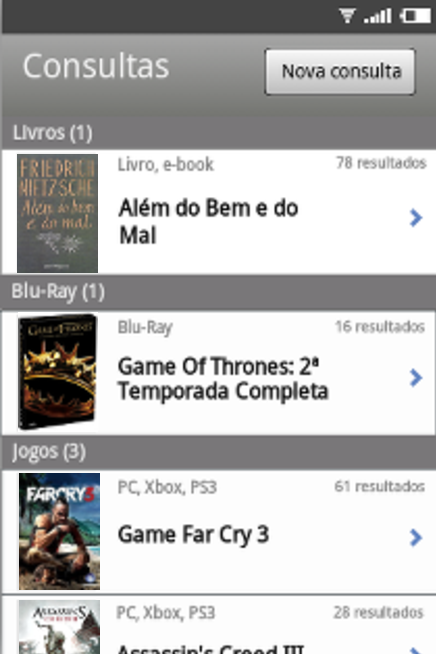
\includegraphics[scale=.71]{tela/TelaHistorico}
    \end{figure}
\end{frame}

% --------------------------------- slide -------------------------------------
\begin{frame}
	\frametitle{Protótipo}
	\framesubtitle{Tela de consulta em andamento}

    \begin{figure}
        \centering
        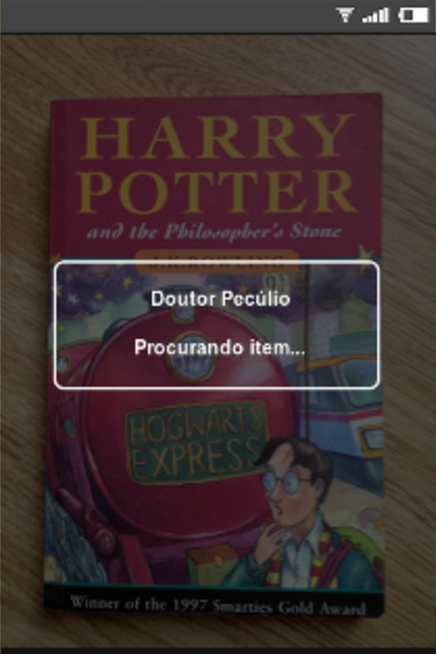
\includegraphics[scale=.71]{tela/TelaBuscando}
    \end{figure}
\end{frame}

% --------------------------------- slide -------------------------------------
\begin{frame}
	\frametitle{Protótipo}
	\framesubtitle{Tela de resultados}

    \begin{figure}
        \centering
        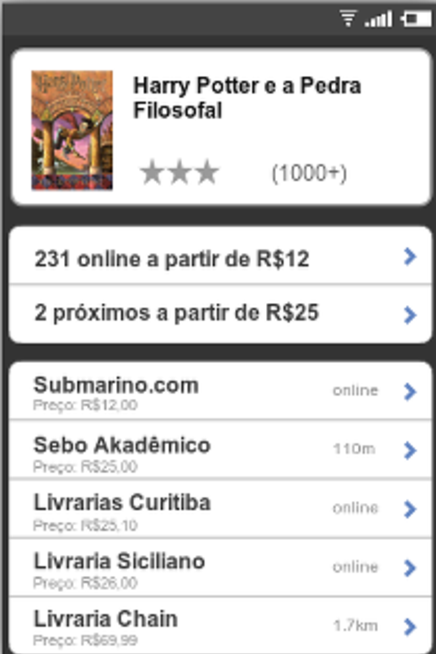
\includegraphics[scale=.71]{tela/Tela}
    \end{figure}
\end{frame}

% --------------------------------- slide -------------------------------------
\begin{frame}
	\frametitle{Protótipo}
	\framesubtitle{Tela de erro ao buscar}

    \begin{figure}
        \centering
        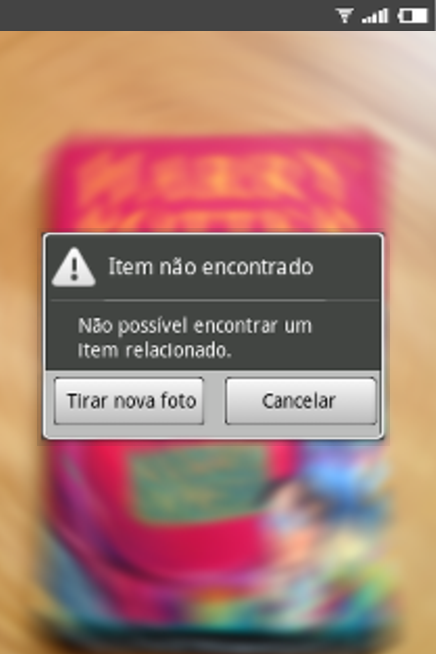
\includegraphics[scale=.71]{tela/TelaErro}
    \end{figure}
\end{frame}

% %%%%%%%%%%%%%%%%%%%%%%%%%%%%%%%% section %%%%%%%%%%%%%%%%%%%%%%%%%%%%%%%%%%%%
% -------------------------------- section ------------------------------------
\section{Avaliação}

% --------------------------------- slide -------------------------------------
\begin{frame}
	\frametitle{Conteúdo}
    \begin{multicols}{2}
        \footnotesize
        \tableofcontents[currentsection,hideothersubsections]
    \end{multicols}
\end{frame}

\subsection{Percurso cognitivo}
% --------------------------------- slide -------------------------------------
\begin{frame}
	\frametitle{Avaliação}
	\framesubtitle{Percurso cognitivo}

    \begin{columns}
        \begin{column}{.6\textwidth}
            Porção do sistema escolhida: Acessar a lista de consultas realizadas.
        \end{column}
        \begin{column}{.4\textwidth}
            \begin{figure}
                \centering
                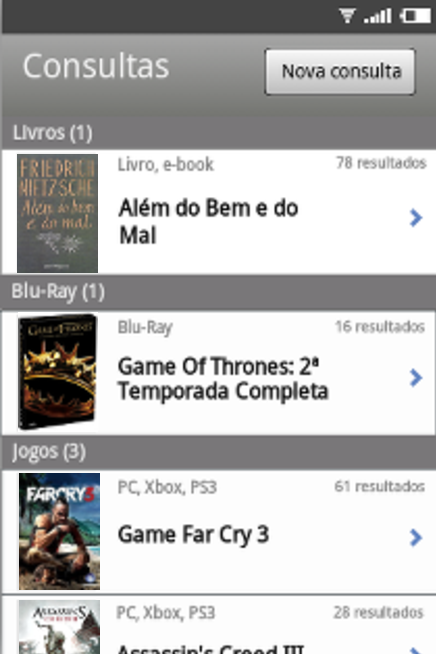
\includegraphics[scale=.5]{tela/TelaHistorico}
            \end{figure}
        \end{column}
    \end{columns}
\end{frame}

% --------------------------------- slide -------------------------------------
\begin{frame}
	\frametitle{Avaliação}
	\framesubtitle{Percurso cognitivo}

    \begin{block}{Passo único}
        Abrir o aplicativo, visualizar a tela inicial.
    \end{block}
    \begin{itemize}
        \item O usuário tentará atingir a meta correta?
        \item O usuário perceberá que a ação correta está disponível na interface?
        \item Uma vez encontrado o elemento de interface, o usuário reconhecerá que ele produzirá o 
efeito desejado?
        \item Após a ação correta ser executada, o usuário perceberá que progrediu em direção à solução 
da tarefa?
    \end{itemize}
\end{frame}

\subsection{Avaliação heurística}
% --------------------------------- slide -------------------------------------
\begin{frame}
	\frametitle{Avaliação}
	\framesubtitle{Avaliação heurística}
    
\par \noindent \textbf{Elemento da interface:} Lista de consultas já realizadas.
\par \noindent \textbf{Localização:} Tela inicial.
\par \noindent \textbf{Heurística violada:} Falta de contraste entre e fundo e cores.
\par \noindent \textbf{Gravidade:} 1 -- cosmético.
\par \noindent \textbf{Recomendação de solução:} Utilizar cores vivas.
\end{frame}

\subsection{Método de Inspeção Semiótica (MIS)}
% --------------------------------- slide -------------------------------------
\begin{frame}
	\frametitle{Avaliação}
	\framesubtitle{Método de Inspeção Semiótica (MIS)}

    \begin{columns}
        \begin{column}{.6\textwidth}
            Avaliação como é comunicação na porção aonde aparece a o item 
            ``Procurando...''.
        \end{column}
        \begin{column}{.4\textwidth}
            \begin{figure}
                \centering
                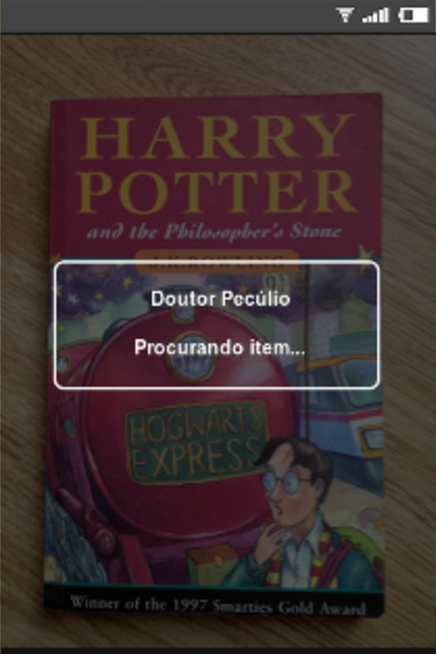
\includegraphics[scale=.5]{tela/TelaBuscando}
            \end{figure}
        \end{column}
    \end{columns}
\end{frame}

\subsection{Método de Avaliação de Comunicabilidade (MAC)}
% --------------------------------- slide -------------------------------------
\begin{frame}
	\frametitle{Avaliação}
	\framesubtitle{Método de Avaliação de Comunicabilidade (MAC)}

	\begin{enumerate}
        \item Preparação;
            \begin{itemize}
                \item Definição: visualizar histórico de buscas;
                \item Participante: Lucas;
                \item Roteiro: Observar por dificuldades;
                \item Teste-piloto: 
            \end{itemize}
        %~ \item Aplicação;
        %~ \item Interpretação;
        %~ \item Consolidação dos resultados;
        %~ \item Relato dos resultados;
	\end{enumerate}
    
    \begin{figure}
        \centering
        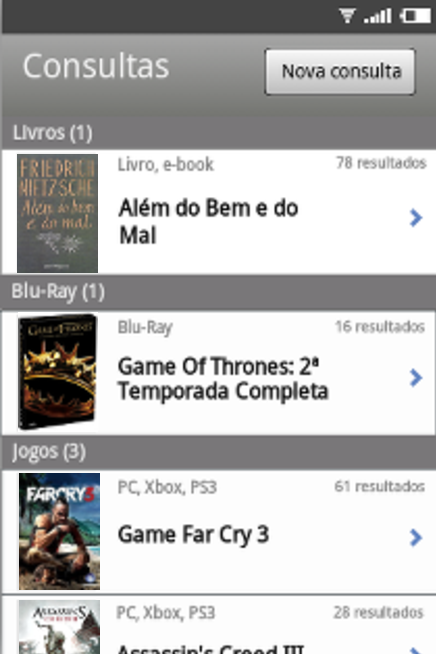
\includegraphics[scale=.45]{tela/TelaHistorico}
    \end{figure}
\end{frame}
% --------------------------------- slide -------------------------------------
\begin{frame}
	\frametitle{Avaliação}
	\framesubtitle{Método de Avaliação de Comunicabilidade (MAC)}

	\begin{enumerate} \setcounter{enumi}{2}
        \item Aplicação;
            \begin{itemize}
                \item Cenário: Abrir o aplicativo doutor pecúlio e visualizar suas consultas já
                        realizadas.
                \item Entrevista pós-teste: Aparece a etiqueta \textsc{Socorro!} Se o usuário não consegue realizar a
                        tarefa.
            \end{itemize}
        %~ \item Interpretação;
        %~ \item Consolidação dos resultados;
        %~ \item Relato dos resultados;
	\end{enumerate}
    
    \begin{figure}
        \centering
        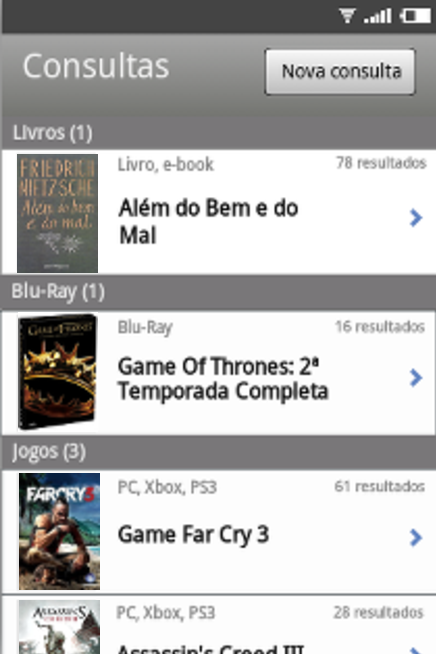
\includegraphics[scale=.4]{tela/TelaHistorico}
    \end{figure}
\end{frame}
% --------------------------------- slide -------------------------------------
\begin{frame}
	\frametitle{Avaliação}
	\framesubtitle{Método de Avaliação de Comunicabilidade (MAC)}

	\begin{enumerate} \setcounter{enumi}{2}
        \item Interpretação;
            \begin{itemize}
                \item Neste ponto podem surgir rupturas de comunicação.
            \end{itemize}
        %~ \item Consolidação dos resultados;
        %~ \item Relato dos resultados;
	\end{enumerate}

        \begin{columns}
           \begin{column}{.4\textwidth}
                \hfill
                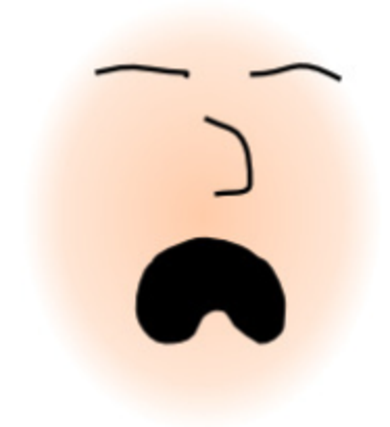
\includegraphics[scale=.3]{imagens/LixoSono}
                \vfill
            \end{column} 
            \begin{column}{.6\textwidth}
                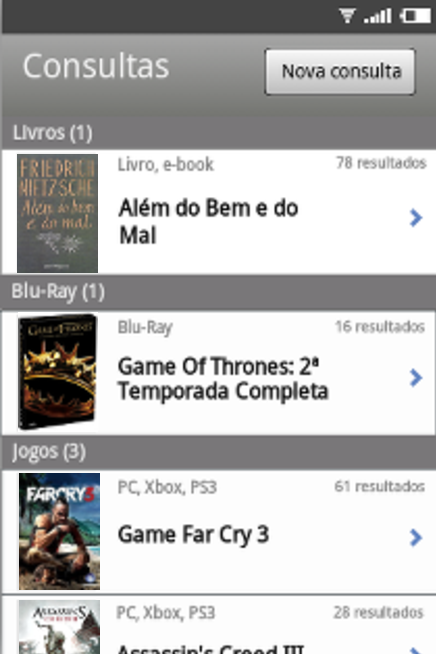
\includegraphics[scale=.5]{tela/TelaHistorico}
            \end{column}
        \end{columns}
\end{frame}

% --------------------------------- slide -------------------------------------
\begin{frame}
	\frametitle{Avaliação}
	\framesubtitle{Método de Avaliação de Comunicabilidade (MAC)}

	\begin{enumerate} \setcounter{enumi}{2}
        \item Consolidação dos resultados;
            \begin{itemize}
                \item O aplicativo não mostra qual foi a última busca,
                apenas listas todas as realizadas.
                \item Todos participantes utilizaram a mesma etiqueta.
            \end{itemize}
        \item Relato dos resultados;
            \begin{itemize}
                \item O objetivo era ver se o usuário iria conseguir saber que aquela porção era relativa a suas 
        últimas pesquisas realizadas, e a conclusão preliminar, visualizando o único caminho, após ter 
        sido aberto o \emph{software}, a etiquetagem resultou em ``socorro'' já que a função não estava 
        evidente e pode dizer ``desisto'' quando pode acreditar que não existe aquela porção do 
        sistema, a sugestão de melhoria seria então colocar um texto dizendo ``últimas consultas''
        antes de aparecerem as últimas consultas do usuário.
            \end{itemize}
        \end{enumerate}
\end{frame}
% %%%%%%%%%%%%%%%%%%%%%%%%%%%%%%%% section %%%%%%%%%%%%%%%%%%%%%%%%%%%%%%%%%%%%
% -------------------------------- section ------------------------------------
\section{Considerações Finais}

% --------------------------------- slide -------------------------------------
\begin{frame}
	\frametitle{Conteúdo}
    \begin{multicols}{2}
        \small
        \tableofcontents[currentsection,hideothersubsections]
    \end{multicols}
\end{frame}
% --------------------------------- slide -------------------------------------
\begin{frame}
	\frametitle{Considerações Finais}

	\begin{block}{Doutor Pecúlio}
	O aplicativo é viável e com diferencial no mercado.
	\end{block}
    
    \begin{block}{Avaliação}
	A avaliação revela que podem haver rupturas de comunicação.
	\end{block}
\end{frame}

% %%%%%%%%%%%%%%%%%%%%%%%%%%%%%%%% section %%%%%%%%%%%%%%%%%%%%%%%%%%%%%%%%%%%%
% ------------------------------ slide ----------------------------------

\section*{Referências}

\begin{frame}{Referências}

	\footnotesize{
	\begin{thebibliography}{99}
	\beamertemplatebookbibitems
	\bibitem[Barbosa]{p1} BARBOSA, Simone D. J.; SILVA, Bruno S. (2010)
	\newblock Interação humano-computador
	\newblock \emph{Editora Campus-Elsevier}, ISBN 978-85-352-3418-3.

	\bibitem[Rocha]{p1} DA ROCHA, H. V.; BARANAUSKAS, M. C. C. (2010)
	\newblock Design e avalia{\c{c}}{\~a}o de interfaces humano-computador
	\newblock \emph{Unicamp}, ISBN 978-85-888-3304-3.
	
	\bibitem[Love]{p1} LOVE, Steve (2005)
	\newblock Understanding mobile human-computer interaction
	\newblock \emph{Elsevier Science}, ISBN 978-00-804-5580-8.
	\end{thebibliography}
	}
%	\beamertemplatearticlebibitems

\end{frame}

\section*{}

\begin{frame}
	\vspace{-15px}
	\begin{center}
		\Huge{Obrigado!}

		\small

		\cyrtext{Спасибо за внимание!}
	\end{center}

	\vspace{15px}
	\small Carlos Alberto Oliveira de Souza Junior \\
	\footnotesize{  \textsl{carlos\_bertojr@hotmail.com} }
	
	\vspace{20px}
	\small Lucas José Campos Lorenzetti \\
	\footnotesize{  \textsl{goodlucas@gmail.com} }
	
	\vspace{20px}
	\small Paulo Roberto Urio \\
	\footnotesize{  \textsl{paulo@bk.ru} }
\end{frame}

\end{document}
